% This is "sig-alternate.tex" V1.8 June 2007
% This file should be compiled with V2.3 of "sig-alternate.cls" June 2007
%
% Layout based on sig-alternate.tex V1.8 example file

\documentclass{sig-alternate}
% \usepackage{url}
\usepackage{hyperref}
\usepackage{natbib}
\usepackage{listings}

% \setlength\fboxrule{0.5pt}


\begin{document}

\CopyrightYear{2009}
\toappear{} % Suppress explicit copyright rights notice.

\title{The Promises and Perils of Mining Ohloh.net}

\numberofauthors{1}
\author{
% 1st. author
\alignauthor Henk Poley\\
  \affaddr{Vrije Universiteit Amsterdam}\\
  \email{hpy300@cs.vu.nl}
}

\date{July 2009}


\maketitle

\begin{abstract}
Ohloh.net is a website that indexes open source software projects, and generates some statistics on their source and committers. In this paper I pose a few scientific use cases for the data exposed through the Ohloh website \& API, and a review of existing papers on this subject.
\end{abstract}


\section{Introduction}
Ohloh was founded by two former Microsoft managers Jason Allen and Scott Collison in 2004. Website launched February 2006. Ohloh contains data on approx. 300.000 projects, and 330.000 source committers.

Ohloh displays several code metrics for the projects it indexes. For example it will display warnings when the code to comment ratio is subpar, or when there are only very few developers. Similarly there are analysis badges for positive points like long running projects with a stable development track.


\subsection{Related websites}
\emph{Sourceforge.net} is a large website that hosts open source projects. Sourceforge has recently (May 2009)acquired Oh\-loh. Changes to either Ohloh or Sourceforge at not worked out yet. Though further orientation on finding projects -on Ohloh's side- and hosting projects -on Sourceforge's side- seems obvious. Ohloh is readying a site relaunch end june, early august 2009 (\cite{behind-the-scenes}).

\emph{Freshmeat.net} is a website that indexes open source pro\-jects since 1998. In comparison to Ohloh there is less emphasis on developers, and more on the projects. Ohloh.net has surpassed Freshmeat.net since November 2008, according to compete.com site analysis. Alexa.com does not show this change. But did show stark changes in their statistics aggregation overall during this time, and should probably not be trusted.

\emph{DistroWatch.com} moves in more or less the same open source space, but collects only high level projects that integrate software together into desktop OSes. This site is less focussed on individual developers, but more on the companies and groups the aggregate their work in distributions. It has about half the visitors as Freshmeat.net, and was surpassed by Ohloh in September 2008 according to compete.com.

On \emph{Advogato.org} developers can register and write a little blurb about themselves. There they can link to projects they worked on. Other registered users can give their opinion about their level of knowledge as a developer (Master, Journeyer, or Apprentice). There seems to be no automated fact aggregation going on, other than displaying contents of RSS feeds from a developer blog.

The major difference to the other sites in this space, is that Ohloh tries to extract facts from the source code itself.


\section{Promises}\label{sec:prom}

Note: Ohloh limits the number of API calls to 1000 per day. Statistical analysis during the project run time was limited by that fact.


\subsection{Promise: Learn what people are using and contributing to}

For registered users Ohloh shows a listing of their projects, as long as the users adds it themselves. For projects with known publicly accessible repositories their personal commit history is shown in abbreviated form.

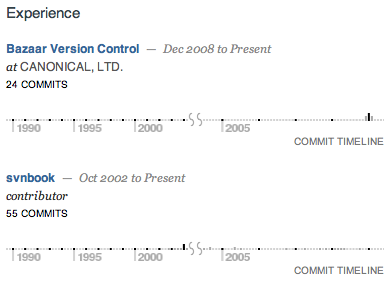
\includegraphics[width=80mm]{Experience.png}

There are also more formal ways to access the data about Ohloh users. In the paper "RDFohloh, a RDF wrapper of Ohloh" \cite{Fernandez:2008p4488}  worked on exposing the accounts on Ohloh as Friend-Of-A-Friend (FOAF) data in RDF format through the Ohloh API.

RFD is an XML based markup language that stores fact triplets, data like \{"Linus Torvalds", "develops", "Linux"\}. Research in artificial intelligence promises that this is a good basis for higher level inferences. Query languages like SPARQL and OWL are developed for this. By picking common words -formalized in "ontologies"- different websites should be able to share facts. Friend-Of-A-Friend (or FOAF) is currently a common use case of RDF. With FOAF you encode the 'knows' relationship, or who knows who.

A problem with this data is that different users in the Ohloh database could well be the same person, see sec. \ref{need-smushing}.

\subsection{Promise: Journaling lets you keep people up-to-date on what you're coding}

This requires the project maintainers to keep a weblog hosted on Ohloh itself. Other people can break into the timeline by mentioning (linking) the project in their posts. There are currently 934 projects with one or more journal entries, either by maintainers or Ohloh users mentioning the project. This means that about 3 promille of the projects have something journaled. A tiny fraction of the total.

Ohloh should consider letting their users add external RSS feeds about their project, automatically aggregating these in the journal posts. Currently RSS feeds are aggregated, but not combined into the journal view.


\subsection{Promise: Increase awareness of your open source projects}
Ohloh promises that having your project on their site increases awareness of the project. People can find projects on the site by using Ohloh's search engine, or by stumbling on them via an interesting user. The project search engine sorts the results by number of accounts that have the project in their stack. This won't give you an opportunity if you project is relatively new with few users. To see if finding a project via contributing people is possible, we look at exposure via high ranked users on Ohloh.

Kudorank starts at 7 after the first pass of their ranking, and declines over time. Only receiving a 'kudo' from someone else's Ohloh account increases this score. This happens either by direct vote, or someone using your project in one of their software 'stacks' \cite{ohloh-kudos}. This means ranks 8 and above are by influential contributors within the Ohloh kudo system.

\begin{tabular}{ r r }
  kudorank & \#contributers \\
  10 &    63 \\
  9  &  3504 \\
  8  & 10583 \\
  7  & 26465 \\
\end{tabular}

With this we can estimate the amount of users with increased exposure at around 14.000 (kudorank 8, 9 \& 10). Set against the total user and committers base of about 330.000 gives us a 4.2\% of the total. This matches with similar metrics like the active blogs survey by Technorati. 5.6\% on a total of 133 million total blogs had at least one post the last 120 days (\cite{blog-state-2008}). Open source is often described as 'scratching an itch' for the individual developer. This data at least supports this notion, in that the abandoning rate of open source projects is similar to life describing projects like a blog. 

New projects should consider having a 'celebrity contributor' on their project if they want increased awareness.

\subsection{Promise: Estimating coding behavior change}
Ohloh indexes commit size on projects with public repositories. Looking at changes in the commit size could give an indication of a coding philosophy change.

This was researched in "Continuous Integration in 
Open Source Software Development" \cite{Deshpande:2008p4463}. Their research hypotheses was: The average commit size in any year is greater than the average commit size during the next year. This was found to be non existant at 95\% confidence level.

Further research could be done by actively looking for interesting strings and code within the Ohloh repository mining backend, see sec. \ref{find-unittest}.


\section{Perils}

\subsection{Peril: One person could be represented as multiple contributors}\label{need-smushing}

A problem with the data from Ohloh is that different committers could be the same person. For example a search for \emph{torvalds} will return 15 results. One is Linus Torvalds own Ohloh account. Another is a fan. And 13 are Linus Torvalds commits to projects that are not linked to his personal account.

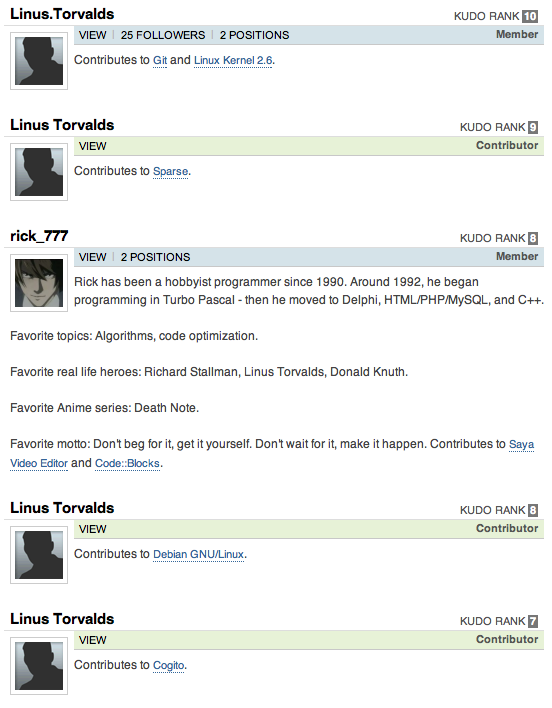
\includegraphics[width=80mm]{TorvaldsSearch.png}

The paper "Smushing RDF instances" \cite{Shi:2008p4464} worked on combining ('smushing') accounts and committers that represent the same person.

The data available on Ohloh is quite sparse. Shi only managed to combine 13 committers on Ohloh, over the 12.613 accounts they had fetched through the API. On mailing lists they could smush at least a few percent of the people. Ohloh could consider mining mailing lists and trying to combine committers based on that, see \ref{sec:mine-ml}.

A possible solution is to use voluntary combinations, where the users can vote on combining contributors from different code bases into one persona. 


\subsection{Peril: Web scraping gets you more info than using API}
During my project it quickly became apparent that the API is only of limited use. Data available to browsers is not seen on their matching .xml file in the API. Most of it can be found, but needs extra trips to the API, quickly dividing the amount of useful data you can access from 1000 API calls (sec. \ref{sec:prom}).

..TODO.. example with HTML

\lstset{language=html}
\begin{lstlisting}
<p>TODO: place your source code here</p>
\end{lstlisting}

..TODO.. example with XML

\lstset{language=xml}
\begin{lstlisting}
TODO: place your source code here
\end{lstlisting}


This is what Ohloh has to say about it themselves: "The design concept is that for each web page on Ohloh, there may be an equivalent XML-formatted version of the page. Currently, only a small subset of the Ohloh site is available as XML, but more data will become available over time." \cite{ohloh-api}. We can conclude that that since 2007 their API still does not cover their entire database.



\subsection{Peril: Can't find people by programming language}
Currently you cannot find people who use one -or several- language(s), without spidering the whole site and scraping it yourself. With the 1000 queries per day limit, one would need about a year (330 days) to scrape the entire user base. I encountered this problem when implementing the algorithm in section \ref{related-devs}.


\subsection{Peril: Commit stats do not show changed lines}

Encountered in "Continuous integration in open source software development" \cite{Deshpande:2008p4463} is the problem that Ohloh only counts the lines that are removed from the previous state, and lines added in the commit. The amount of overlap between added and removed lines is unknown, there is no count of which lines are only slightly changed. The lines changed or overlap measure could be used to asses code churn. ..TODO..


\section{Advice to Ohloh}
Some interesting additions the people at Ohloh could add to their scraper or analyses backend.


\subsection{Mine mailinglists}\label{sec:mine-ml}

Ohloh should consider mining mailing lists and using this to combine their user accounts. Though there is of course no protocol for showing which committer name a mailing list member has, registered users at Ohloh need to supply at least one email address. This could be used to find the registered accounts back in the mailinglists. Ohloh could then add their contribution to a project, without knowing their commit history.


\subsection{Find copied libraries \& frameworks}
Some development frameworks require you to copy over some or all of their code in your project before you can use them. Ohloh could has files and try to find where the common ones originate. This would need a second pass over the source files though.

Excluding duplicated code would lead to fairer project source code statistics. And could help with the smushing problem in sec. \ref{need-smushing}, by listing projects that used someone's code on their own profile.


\subsection{Show related developers for your project}\label{related-devs}

A nice idea for Ohloh would be to show other people who might be able to help with your project. The proposed algorithm:

\begin{enumerate}
  \item Collect programming language(s) used by your project
  \item Find programmers who can program (all) these languages
  \item Remove inactive programmers
  \item Remove over-active programmers
\end{enumerate}

I have written some -incomplete- Python code to support this. It is available at Google Code (\cite{pyanohloh}). A problem I had in mining the data was that you can't find all programmers by the languages they use. Though if I had started right away with caching data from Ohloh regardless if I knew what to do with it, I might have had a big enough cache of user-data to show some results with this algorithm.

Even the most used languages like C or Java end up being used in about 15\% of the commits. Scripting languages like PHP or Python are at about 8\%. Real time collection of data (up to a 1000 language-person pairs) would give you around 100 people per language. From which then a subsection needs to be found. And this subsection can't be found with the data from a single API call per contributor. Since this only returns the single top language of a programmer, further reducing the amount of data you can get out of Ohloh directly.

\subsection{Find good programmers}

..TODO..

Can find \emph{popular} programmers.

Many programmers, so 1000 query limit (sec. \ref{sec:prom}) is a factor.

Commits that shrink the codebase (cite?).

Commits that fix bugs, look for common ticket references.

Ohloh could graph developer connections outside of the kudo-givers graph. This needs smushing, so further  analyses.


\subsection{Find unit-tests}\label{find-unittest}
In 'Continuous Integration in Open Source Software Development' \cite{Deshpande:2008p4463} they tried to infer if continuous integration occurred more in open source projects since the widespread introduction of testing paradigms. With the limited data from Ohloh they could not find a change in behavior.

Instead Ohloh could look for testing inside the code bases it mines. A good first approximation would be to just look for files with the string 'text' in their name. Most projects use on of the xUnit derived test frameworks, which follow common terminology. Looking for files with commonly used strings in unittests like 'setup', 'teardown' and 'fixture' would be a good second order approximation.

Ohloh currently does not show the filenames used inside the commits, so this kind of analyses needs a trip to the individual repositories.


\subsection{Integrate software attention measurements}
There are websites like IUseThis.com, Wakoopa.com and Debian Popularity Contest that measure software use. Either by voluntary votes or direct measurement. Importing this data could show a better picture of actual open source software use.


\subsection{Scrape bugtrackers}
Like mailinglists, bugtrackers contain information about the development of a project. Unlike mail, this is more formalized. Often it is protocol to mention the bug number that is fixed by the commit. By tracking these as links into the bugtracker, research like "When Do Changes Induce Fixes?" \cite{Liwerski:2005p4574} could be run on a regular basis. Developers can then be compared on the basis of amount of fixed bugs versus bug introducing fixes.


\section{Conclusions}

..TODO..

I will send all my suggestions to the Ohloh forum, and look forward to the relaunch of their website.


\section{Acknowledgments}
The project supervisor is Rahul Premraj. The second reader of this paper is Hans van Vliet. The structure of the paper was inspired by "The Promises and Perils of Mining Git" \cite{Bird:2009p4462}. 


\bibliographystyle{plainnat} % {abbrv}
\bibliography{myrefs}
%\bibliography{webrefs} % Meh, adds another References section..

\end{document}
